%\documentclass[notes]{beamer}       % print frame + notes
%\documentclass[notes=only]{beamer}   % only notes
\documentclass{beamer}              % only frames
\usepackage[default]{sourcesanspro}
\usepackage[ngerman]{babel}
\usepackage[utf8]{inputenc}
\usepackage{graphicx}
\usepackage{ccicons}
\usepackage{listings}
\usepackage{amsmath}
\lstset{basicstyle=\scriptsize\ttfamily}
\usetheme{default}
\usebeamercolor{wolverine}
\useoutertheme{smoothbars}

\beamertemplatenavigationsymbolsempty{}

\setbeamertemplate{footline}[text line]{%
  \parbox{\linewidth}{\vspace*{-8pt}OS: Künstliche Intelligenz und Software Engineering - Prof. Andreas Both - Sommersemester 2024 - HTWK Leipzig\hfill\insertpagenumber}}

\setbeamercolor{title}{fg=black}
\usepackage[inkscapearea=page]{svg}
\usepackage[edges]{forest}
\usepackage{longtable,booktabs} %Tabellen mit zeilenumbruch
\usepackage{subcaption}
\definecolor{LightGray}{rgb}{0.97,0.97,0.97}
\definecolor{codegreen}{rgb}{0,0.6,0}
\definecolor{codegray}{rgb}{0.5,0.5,0.5}
\definecolor{codepurple}{rgb}{0.58,0,0.82}


\title{Sicherung der Korrektheit von durch LLMs erzeugtem Code}

\author{Istvan J. Mocsy}
\subtitle{OS: Künstliche Intelligenz und Software Engineering - Prof. Andreas Both - Sommersemester 2024 - HTWK Leipzig}
\date{\today}
\begin{document}

{
	\usebackgroundtemplate{%
			
\includegraphics[width=\paperwidth]{images/balkengreen.png}
		}
\begin{frame}[plain]

\includegraphics[height=3ex]{images/HTWK_Zusatz_de_H_Black_K.eps}
 \titlepage{}
 \cczero
\end{frame}
}

\makeatletter
\patchcmd{\endbeamer@frameslide}{\ifx\beamer@frametitle\@empty}{\iffalse}{}{\errmessage{failed to patch}}
\makeatother

\makeatletter
\setbeamertemplate{frametitle}{%
	\ifbeamercolorempty[bg]{frametitle}{}{\nointerlineskip}%
	\@tempdima=\textwidth%
	\advance\@tempdima by\beamer@leftmargin%
	\advance\@tempdima by\beamer@rightmargin%
	\begin{beamercolorbox}[sep=0.0cm,left,wd=\the\@tempdima]{frametitle}
		\raisebox{-0.15cm}{
\includegraphics[width=0.0212\paperwidth]{images/headergreen.png}}
		\begin{minipage}{.81\paperwidth}
			\usebeamerfont{frametitle}%
			\vbox{}\vskip-1ex%
			\if@tempswa\else\csname beamer@fteleft\endcsname\fi%
			\strut\insertframetitle\par%
			{%
				\ifx\insertframesubtitle\@empty%
				\else%
				{\usebeamerfont{framesubtitle}\usebeamercolor[fg]{framesubtitle}\strut\insertframesubtitle\par}%
				\fi
			}%
		\end{minipage}%
		\enspace\quad\qquad\raisebox{-0.15cm}{
\includegraphics[width=0.0212\paperwidth]{images/headergreen.png}}
		\if@tempswa\else\vskip-.3cm\fi% set inside beamercolorbox... evil here...
	\end{beamercolorbox}%
}
\addtobeamertemplate{footnote}{}{\vspace{2ex}}
\makeatother

\section{Motivation}
\begin{frame}{Problemstellung}
	\begin{columns}
	\column{.5\linewidth}
Problem: Output von LLMs nicht immer verlässlich.

\vspace{30mm}

Motivation: Es soll sichergestellt sein, dass durch LLMs erzeugter Code korrekt ist.
    \column{.5\linewidth}
        \begin{figure}
        \centering
        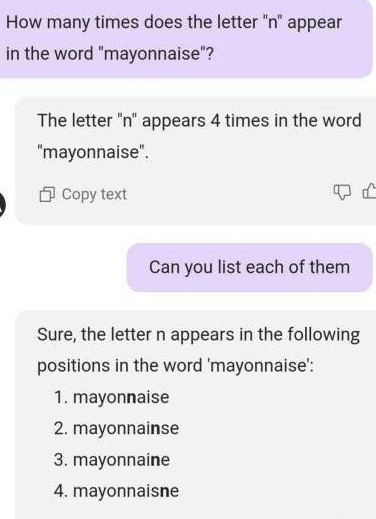
\includegraphics[width=0.35\paperwidth]{images/mayonnaise.png}
        \caption{Künstliche Intelligenz?\cite{mayonnaise:reddit}}
        \label{fig:stry}
    \end{figure}
    \end{columns}
\end{frame}

\begin{frame}{Fehlerhafter Code}
    \begin{figure}
        \centering
        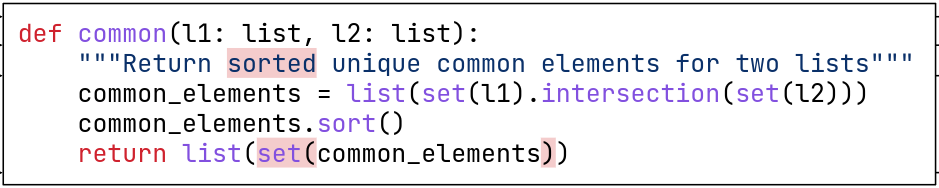
\includegraphics[width=0.8\paperwidth]{images/sortedlistwrongnoHE.png}
        \caption{Von ChatGPT erzeugter inkorrekter Code\cite{liu2024your}}
    \end{figure}
\end{frame}
\begin{frame}{Fragestellung}

\centering Wie kann man die funktionale Korrektheit von durch LLMs erzeugtem Code messen?

\end{frame}

\begin{frame}{Motivation - funktionale Korrektheit von Code}
Zur Messung der Korrektheit bedarf es einer Auswahl...
\begin{itemize}
    \item ... von zu testenden LLMs zur Erzeugung von Code
    \item ... einer geeigneten Methode zum Benchmarking
    \item ... geeigneter Metriken zur Bewertung
\end{itemize}
\end{frame}

\begin{frame}{Rückblick}
\begin{itemize}
    \item 2021 noch überwiegend Benchmarking durch Vergleich mit Musterlösung(BLEU)\cite{chen2021evaluating}
    \item Problematik hier bekannt und 2020 näher untersucht\cite{ren2020codebleu}
    \item Benchmarking über Unit Tests\cite{osti_10195511}\cite{chen2021evaluating}
\end{itemize}
\end{frame}

\section{HumanEval}
\begin{frame}{Was ist HumanEval?}
HumanEval\footnote{https://github.com/openai/human-eval} ist ein Benchmarkingframework, welches einen aus 164 Programmierchallenges bestehenden Datensatz beifügt\cite{chen2021evaluating}. Jede dieser Challanges beinhaltet
\begin{itemize}
    \item Signatur der Funktion
    \item Docstring zur Beschreibung der Anforderungen
    \item Beispiele für Input und korrektem Output
    \item Ground-Truth-Implementation
    \item Unit Tests passend zur Signatur
\end{itemize}
\end{frame}

\begin{frame}[fragile]{HumanEval: Promt}
    \begin{lstlisting}
    def common(l1: list, l2: list):
    """Return sorted unique common elements for two lists.
    >>> common([1, 4, 3, 34, 653, 2, 5],
               [5, 7, 1, 5, 9, 653, 121])
    [1, 5, 653]
    >>> common([5, 3, 2, 8], [3, 2])
    [2, 3]"""
    \end{lstlisting}
\end{frame}
\begin{frame}[fragile]{HumanEval: Ground-Truth-Implementierung}
  \begin{lstlisting}
    ret = set()
    for e1 in l1:
        for e2 in l2:
            if e1 == e2:
            ret.add(e1)
    return sorted(list(ret))
   \end{lstlisting}
\end{frame}
\begin{frame}[fragile]{HumanEval: Test}
    \begin{lstlisting}
    METADATA = {}
    def check(candidate):
    assert candidate([1, 4, 3, 34, 653, 2, 5],
                     [5, 7, 1, 5, 9, 653, 121]) == [1, 5, 653]
    assert candidate([5, 3, 2, 8], [3, 2]) == [2, 3]
    assert candidate([4, 3, 2, 8], [3, 2, 4]) == [2, 3, 4]
    assert candidate([4, 3, 2, 8], []) == []"
    \end{lstlisting}
\end{frame}

\begin{frame}{Metrik zur Messung}
Genutzt wird die Metrik pass@k. Per Problem werden k Samples erzeugt. Ein Problem gilt als gelöst, wenn min. ein Sample ein korrektes Ergebnis erzeugt. Anschließend wird der Gesamtanteil der gelösten Probleme berechnet. HumanEval nutzt diese Metrik mit der Anpassung, dass immer n=200 Samples erzeugt werden.
    \begin{figure}
        \centering
        
\includegraphics[width=0.6\paperwidth]{images/passk.png}
        \caption{pass@k - Variante von HumanEval\cite{chen2021evaluating}}
    \end{figure}
\end{frame}

\begin{frame}{Ergebnisse}
Zur Durchführung eines ersten Benchmark-Tests mit HumanEval standen folgende LLMs zur Auswahl
\begin{table}[]
\begin{tabular}{|l|l|l|l|}
\hline
\textbf{Modell} & \textbf{Parameter} & \textbf{Datum} & \textbf{Trainingsdaten} \\ \hline
GPT-Neo\cite{black2021gptneo} & 125M-2,7B & März 2021 & the Pile\cite{gao2020pile}  \\ \hline
GPT-J\cite{wang2021gptj} & 6B & Juni 2021 & the Pile  \\ \hline
TabNine\footnote{https://www.tabnine.com/} &  & Mai 2021 & \\ \hline
Codex & 12M-12B & Mai 2020 & 54 Mio Python GitHub Repos \\ \hline
\end{tabular}
\end{table}
\end{frame}

\begin{frame}{Ergebnisse}
    \begin{figure}
        \centering
        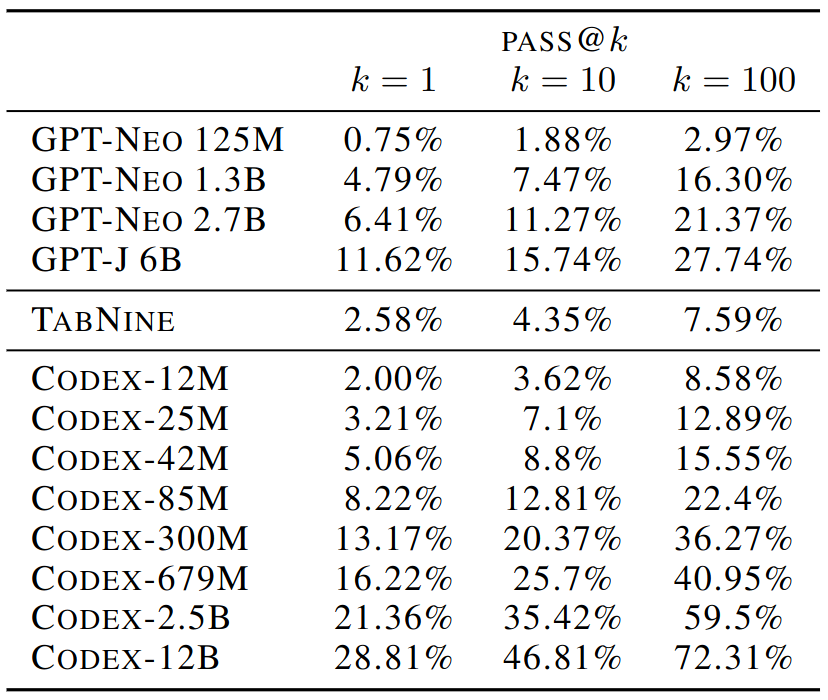
\includegraphics[width=0.55\paperwidth]{images/humanevaleval.png}
        \caption{Ergebnisse des Benchmarks mit k = 1/10/100\cite{chen2021evaluating}}
    \end{figure}
\end{frame}

\section{Codex}
\begin{frame}{Vorstellung Codex}
GPT-3-Modell spezialisiert auf Codeerzeugung mit folgenden Eigenschaften:\cite{chen2021evaluating}
\begin{itemize}
    \item Trainingsdatensatz im Mai 2020 zusammengestellt
    \item Pythoncode aus 54 Mio Repositories(Github)
    \item 159GB in Python-Dateien <1MB
    \item Filterung von autogenerierten Inhalten und z.B. Quellcode mit mehr als 1000 Zeilen
    \item Insgesamt trainiert mit bis zu 12B Parametern
\end{itemize}
\end{frame}

\begin{frame}[fragile]{Vorstellung Codex}
\begin{itemize}
    \item 100B Tokens
    \item Adam optimizer (\(\beta\) 1 = 0.9, \(\beta\) 2 = 0.95, \(\epsilon\) = $10^{-8}$, weight decay coefficient = 0.1)
    \item 175 step linear warmup
    \item Cosine learning rate decay

\end{itemize}
\end{frame}

\begin{frame}{Varianten}
\begin{itemize}
    \item Codex-S\cite{chen2021evaluating}
    \begin{itemize}
        \item Modell mit spezialisierteren Trainingsdaten
        \item Nutzt Trainingsdaten aus Programmierwettkampf und Projekte mit CI
    \end{itemize}
    \item Codex-D\cite{chen2021evaluating}
    \begin{itemize}
        \item Modell zur Erzeugung von Docstrings aus Codebeispielen
        \item Auswertung der Samples per Hand
    \end{itemize}
\end{itemize}
\end{frame}

\begin{frame}{Wahl der Temperatur}
    \begin{figure}
        \centering
        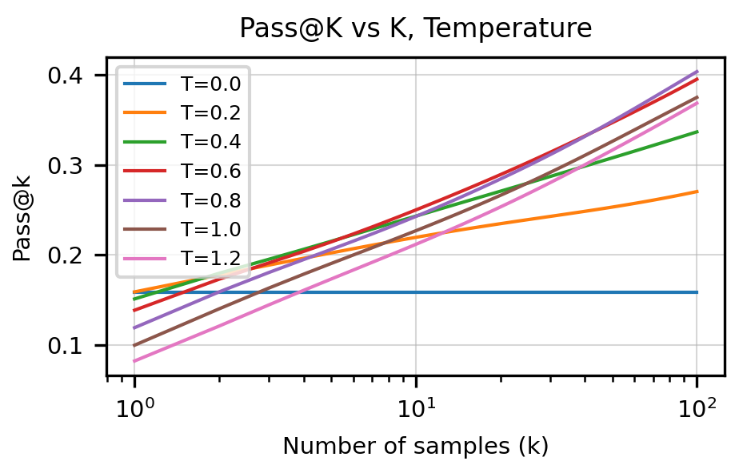
\includegraphics[width=0.7\paperwidth]{images/passkvstemp.png}
        \caption{Verteilung der unterschiedlichen Temperaturen bei verschiedenen k\cite{chen2021evaluating}}
    \end{figure}
\end{frame}

\begin{frame}{Faktor Modellgröße}
    \begin{figure}
        \centering
        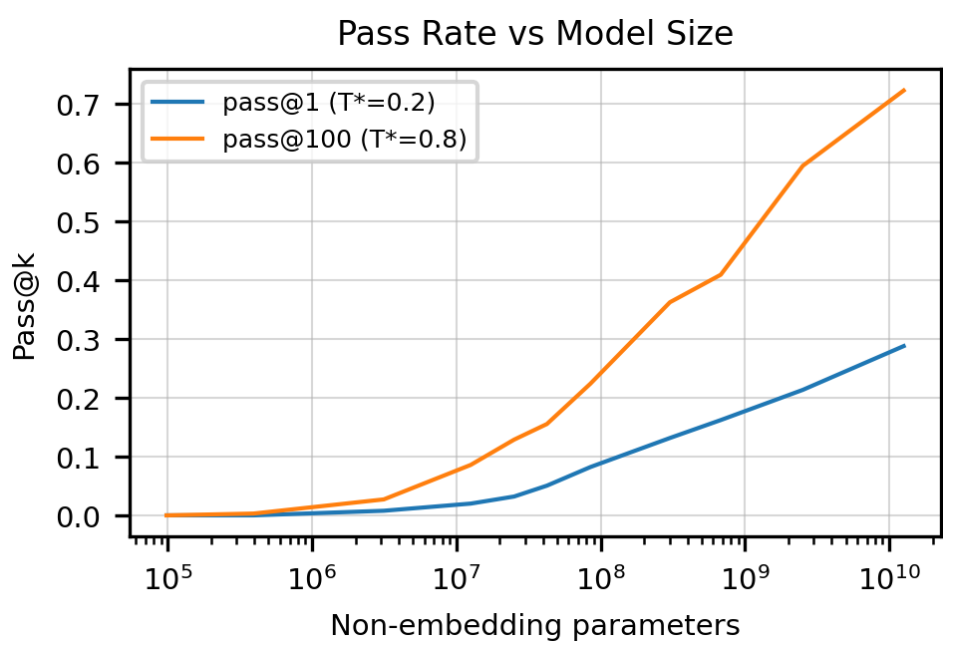
\includegraphics[width=0.7\paperwidth]{images/passkvssize.png}
        \caption{Einfluss der Modellgröße auf pass@k\cite{chen2021evaluating}}
    \end{figure}
\end{frame}

\begin{frame}{Auswahl der Samples bei angepasstem pass@k}
    \begin{figure}
        \centering
        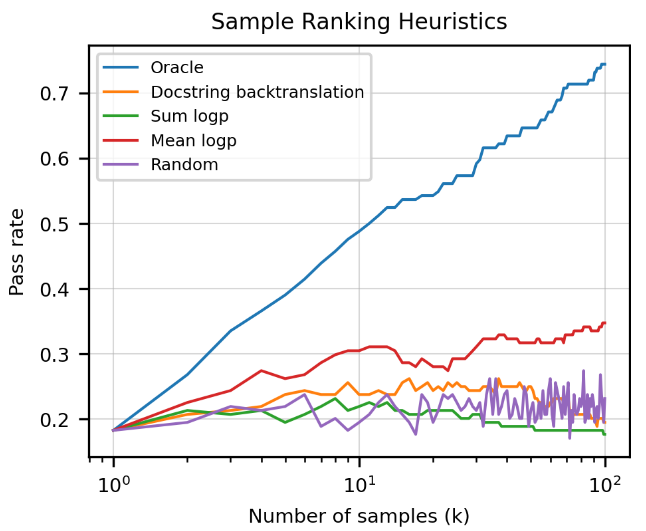
\includegraphics[width=0.55\paperwidth]{images/heuristcs.png}
        \caption{Auswahlmöglichkeiten der Samples im Vergleich\cite{chen2021evaluating}}
    \end{figure}
\end{frame}

\begin{frame}{Limitationen}
\begin{itemize}
    \item Probleme bei zu langen Docstrings mit multiplen Anweisungen
    \item Inkorrekter Code bei korrektem Docstring, aber inkorrekten Beispieloutputs
\end{itemize}
\end{frame}

\begin{frame}{Limitationen}
    \begin{figure}
        \centering
        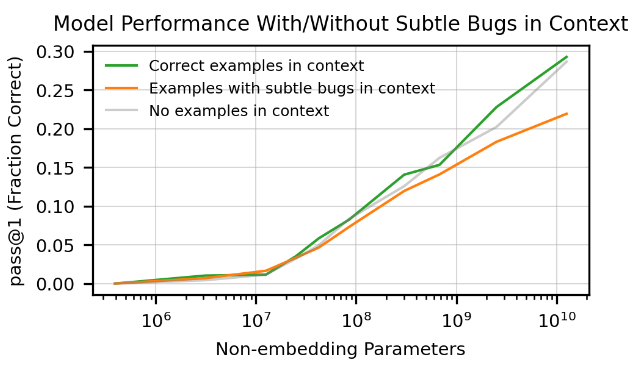
\includegraphics[width=0.6\paperwidth]{images/bugsinexamples.png}
        \caption{Performance der Modelle bei Einführung subtiler Bugs in die Outputmenge\cite{chen2021evaluating}}
    \end{figure}
\end{frame}

\section{EvalPlus}
\begin{frame}{Was ist EvalPlus?}
Generalisiertes Framework, welches bestehende Benchmarks erweitert\cite{liu2024your}
\begin{itemize}
    \item Erweiterung der Testfälle um vielfaches
    \item Nutzung von LLMs und type-aware Mutation zur Testfallgenerierung
    \item Testsuitereduktion für kostengünstigere Ausführung
    \item Auswertung durch diffential testing\cite{mckeeman1998differential}
\end{itemize}
\end{frame}

\begin{frame}{Aufbau EvalPlus}
    \begin{figure}
        \centering
        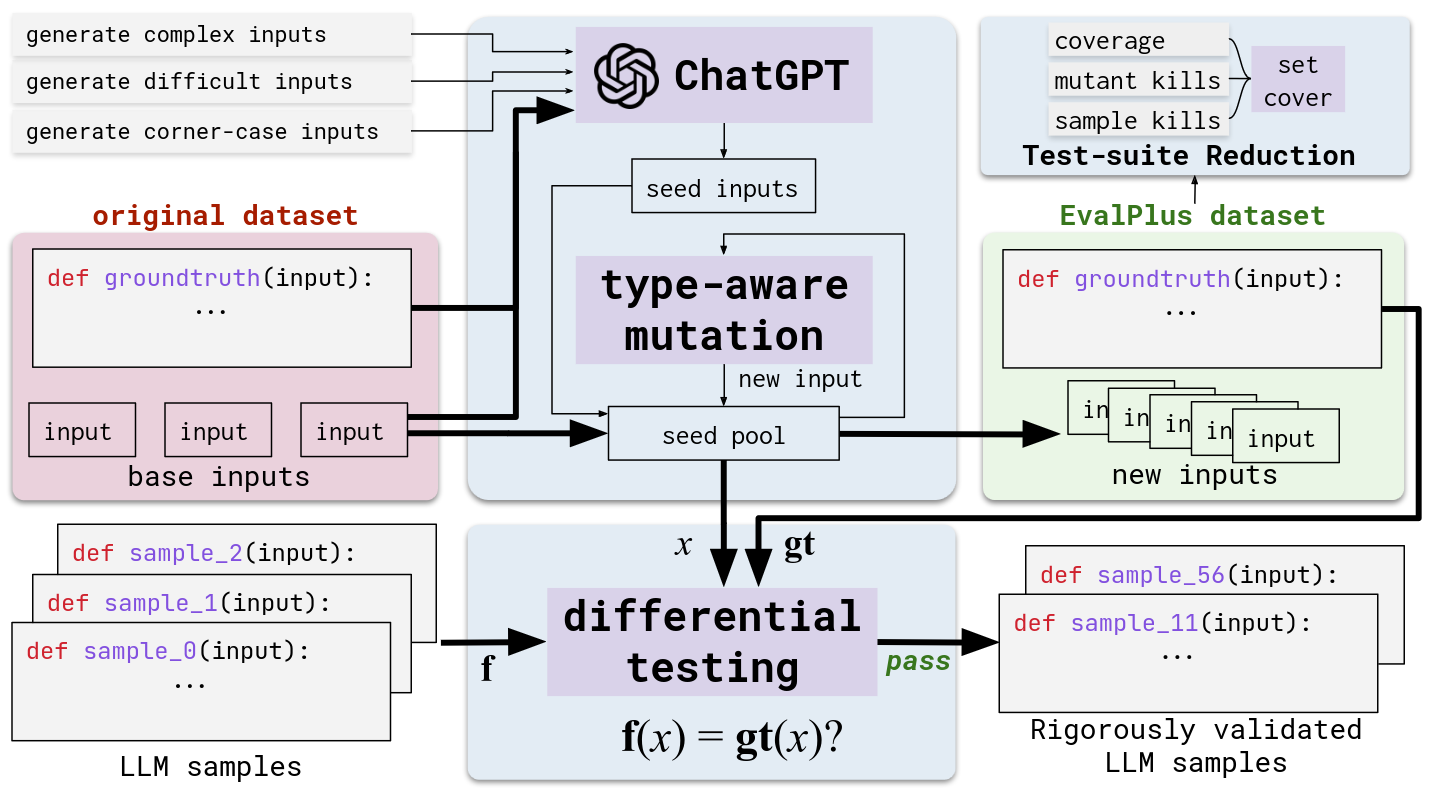
\includegraphics[width=0.8\paperwidth]{images/overviewEplus.png}
        \caption{Überblick über die Struktur von EvalPlus\cite{chen2021evaluating}}
    \end{figure}
\end{frame}

\begin{frame}{Idee: HumanEval+}
Auf HumanEval angewendet, werden mit EvalPlus die Testsuites HumanEval+ sowie HumanEval+-Mini zu erzeugt
    \begin{figure}
        \centering
        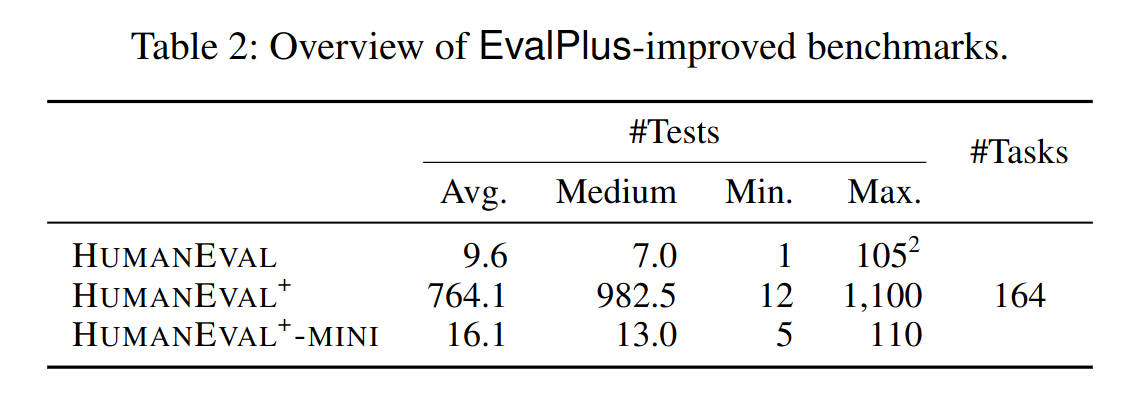
\includegraphics[width=0.6\paperwidth]{images/humanevalbenchmarkbulk.png}
        \caption{Überblick der Benchmark-Verbesserungen durch EvalPlus\cite{liu2024your}}
    \end{figure}
\end{frame}

\begin{frame}{Probleme mit HumanEval: Falsch bewertete Korrektheit}
    \begin{figure}
        \centering
        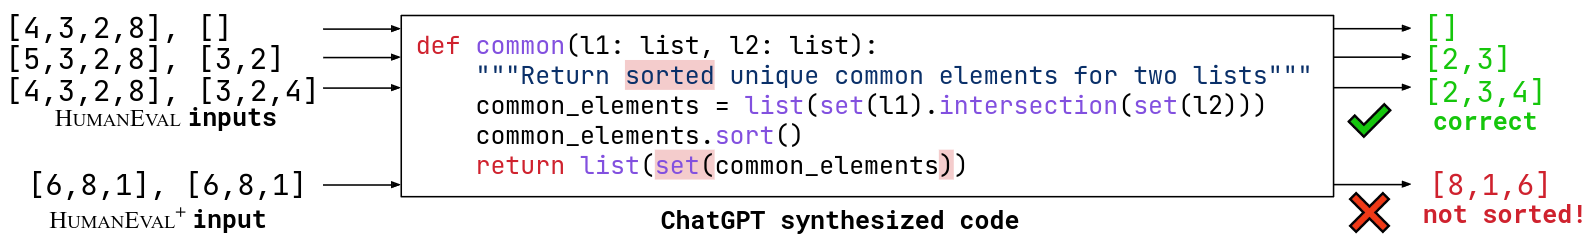
\includegraphics[width=0.8\paperwidth]{images/sortedlistwrong.png}
        \caption{Mit HumanEval-Inputs als korrekt bewerteter Code\cite{liu2024your}}
    \end{figure}
\end{frame}

\begin{frame}{Probleme mit HumanEval: Falsch implementierte Ground-Truth}
    \begin{figure}
        \centering
        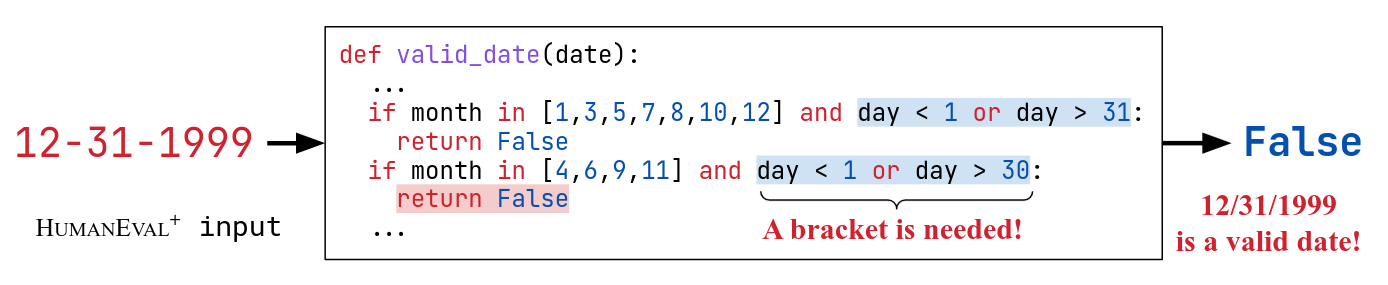
\includegraphics[width=0.8\paperwidth]{images/groundtruthwrong.png}
        \caption{In HumanEval inkorrekt implementierte Ground-Truth\cite{liu2024your}}
    \end{figure}
\end{frame}

\begin{frame}{Ergebnisse der LLMs mit pass@100 > 50}
    \begin{figure}
        \centering
        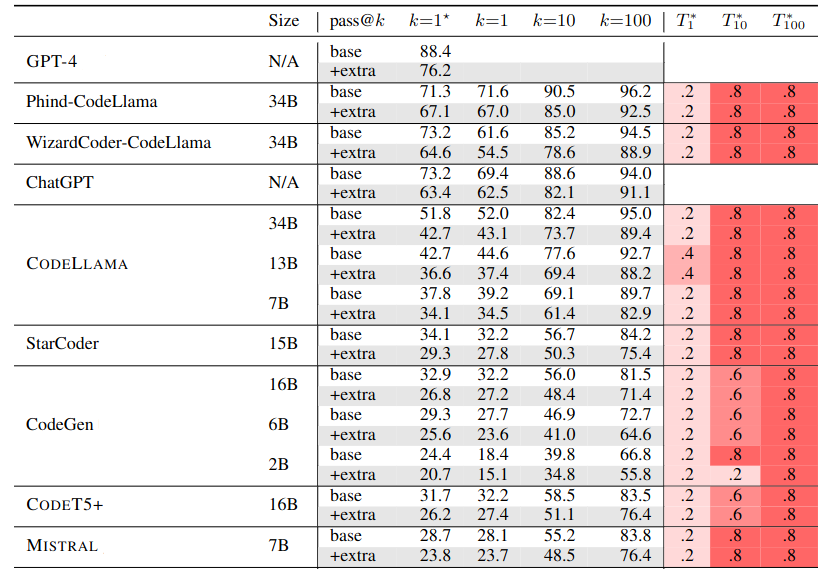
\includegraphics[width=0.7\paperwidth]{images/resultshumaneval+.png}
        \caption{Ergebnisse der einzelnen LLMs im Vergleich\cite{liu2024your}}
    \end{figure}
\end{frame}

\begin{frame}{Vergleich der Ergebnisse über alle Probleme}
    \begin{figure}
        \centering
        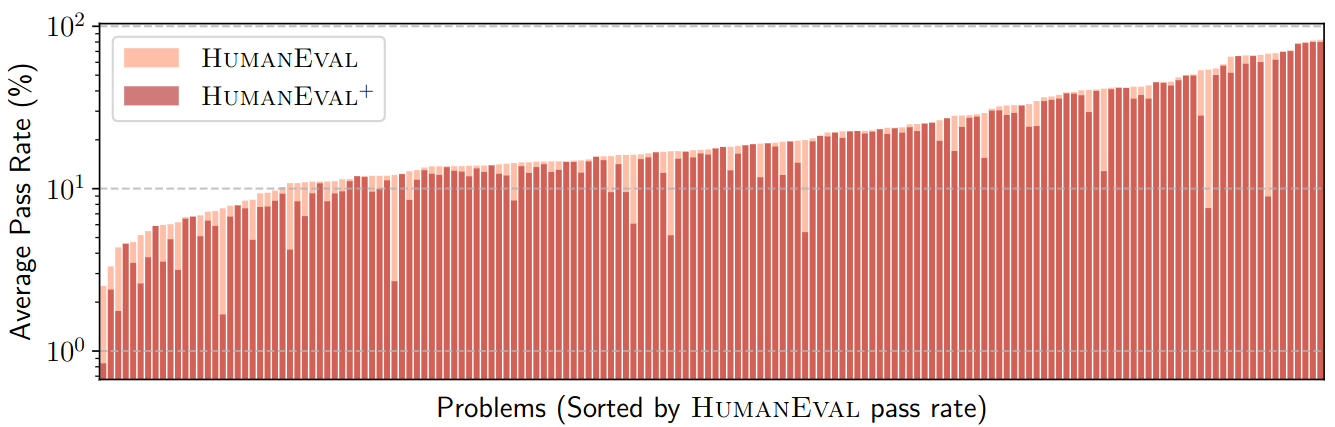
\includegraphics[width=0.8\paperwidth]{images/evalandevalpluscompare.png}
        \caption{Pass-rates über alle getesteten LLMs unter Nutzung von HumanEval und HumanEval+\cite{liu2024your}}
    \end{figure}
\end{frame}

\begin{frame}{Testsuite-Reduktion}
Reduzierung der Ausführungskosten mit folgenden Methoden\cite{liu2024your}
\begin{itemize}
    \item Minimierung der Tests auf ein Subset, welches identische Code-Coverage aufweist
    \item Testen von mutiertem Code, welcher die effektivsten Testfälle zeigt
    \item LLM Sample killings
\end{itemize}
Dies führt im Fall HumanEval+ zu einer Testsuitereduktion des Faktors 47
\end{frame}

\begin{frame}{Ergebnisse HumanEval+-Mini}
    \begin{figure}
        \centering
        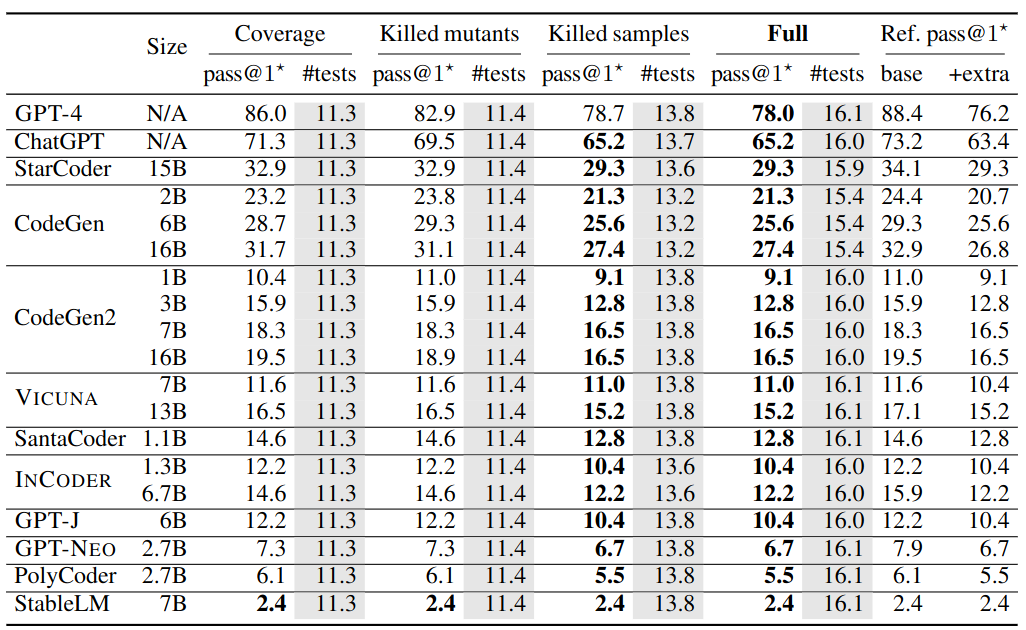
\includegraphics[width=0.8\paperwidth]{images/reducedresults.png}
        \caption{Ergenbisse des Benchmarks mit HumanEval+-Mini unter verschiedenen Reduktionsstrategien\cite{liu2024your}}
    \end{figure}
\end{frame}

\section{Zusammenfassung}
\begin{frame}{Zusammenfassung}
\begin{itemize}
    \item Vorstellung von Verfahren HumanEval, welches Korrektheit von durch LLMs erzeugtem Code messbar macht
    \item Überblick über eine der bewerteten LLMs
    \item Vorstellung von EvalPlus, einem Framework zur Verbesserung von bestehenden Benchmarks
\end{itemize}
\end{frame}

\begin{frame}{Ähnliche Arbeiten}
\begin{itemize}
    \item CodeBleu: Anpassung des Bleuscores auf Code durch Berücksichtigung von AST und Codesemantik\cite{ren2020codebleu}
    \item MBPP(Mostly Basic Programming Problems): Crowd-Sourcing-Projekt mit 974 Programmierproblemen\cite{austin2021program}
    \item MultiPL-E: Erweiterung der Probleme von HumanEval und MBPP auf 18 Programmiersprachen\cite{cassano2023multipl}

\end{itemize}
\end{frame}

\begin{frame}{Ausblick}
\begin{itemize}
    \item Verbesserung der Codeerzeugung durch LLMs durch Wettkampf\footnote{https://evalplus.github.io/leaderboard.html}
    \item Erweiterung von Benchmarks bereits im Gang(HumanEval-X\cite{zheng2023codegeex} for C++, JS und Go, MultiPL-E)
\end{itemize}
\end{frame}

\begin{frame}{Bewertung}
\begin{itemize}
    \item Benchmarking über Unit Tests welches auf den ersten Blick gute Resultate liefert
    \item Struktur erlaubt einfache Erweiterung und Granulierung des Testprozesses
    \item Noch ein sehr weiter weg zum "perfekten" LLM
\end{itemize}
\end{frame}

\section{Quellen}
\begin{frame}[allowframebreaks]
        \frametitle{Quellen}
        \bibliographystyle{abbrv}
        \bibliography{bibliography}
\end{frame}

\section{Lizenz}
\begin{frame}{}
   \centering Diese Belegarbeit ist unter der CC0 1.0 Universal lizensiert. \url{https://creativecommons.org/publicdomain/zero/1.0/}
\end{frame}
\end{document}

% {Copypasta für Bilder, weil man die Syntax eh jedes mal googled wie ein verdammter Ersti}:

% \begin{frame}
% 	\begin{columns}
% 	\column{.5\linewidth}
%     \begin{figure}
%         \centering
%         \includegraphics[width=0.35\paperwidth]{intent.png}
%         \caption{Beispiel Intent}
%         \label{fig:intt}
%     \end{figure}
%     \column{.5\linewidth}
%         \begin{figure}
%         \centering
%         \includegraphics[width=0.35\paperwidth]{rasastory.png}
%         \caption{Beispiel Story}
%         \label{fig:stry}
%     \end{figure}
%     \end{columns}
% \end{frame}


% {Copypasta für Codeblocks, weil man die Syntax eh jedes mal googled wie ein verdammter Ersti}:

% \begin{frame}[fragile]
% \frametitle{Beispiel Taxifahrt-Daten}
% \rule{\textwidth}{1pt}
% \tiny
% \begin{minted}{python}
% def extract_taxi_data() -> [[str, pd.DataFrame]]:
%     dfs_taxi_data = []

%     for taxi_type in config.TAXI_TYPES:
%         df_taxi_type: pd.DataFrame = pd.DataFrame()

%         for year in config.TAXI_YEARS:
%             filename = str(year) + "_" + taxi_type + ".csv"
%             df_year = pd.read_csv(path.join(config.DATA_PATH, filename))

%             df_taxi_type = pd.concat([df_taxi_type, df_year], ignore_index=True)
%             logger.success("{filename} extracted.", filename=filename)

%         dfs_taxi_data.append([taxi_type, df_taxi_type])

%     logger.success("Taxi data extracted.")
%     return dfs_taxi_data
% \end{minted}
% \rule{\textwidth}{1pt}
% \end{frame}
